\section{Démarche Expérimentale}






\begin{minipage}{\linewidth}
    \begin{wrapfigure}{R}{0.4\linewidth}
        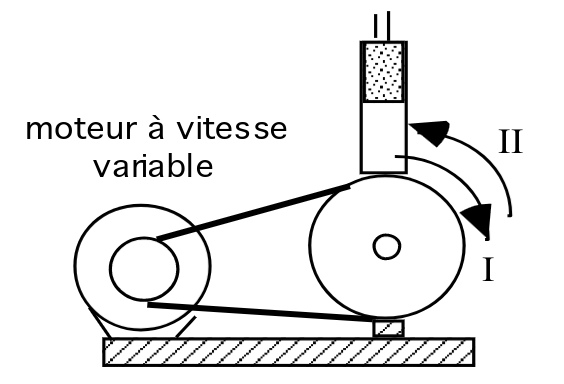
\includegraphics[width=\linewidth]{figures/machine-frigo.png}
        \caption{Schéma du moteur de Stirling comme machine frigorifique \cite{notice}}
        \label{fig:machine_frigo}
    \end{wrapfigure}

    \paragraph*{Machine frigorifique}
    Lors de cette expérience le fonctionnement du cycle de Stirling en machine frigorifique est le point d'intérêt. Il s'obtient en tournant l'arbre de rotation à l'aide d'un moteur externe dont il est possible de mesurer la puissance fournie \(P_{moteur}\) par mesure de sa tension et de son courant d'entrée. Il est important de faire tourner dans ce cas le cycle dans le même sens que lors du fonctionnement moteur afin d'évacuer la chaleur de la tête de mesure, cela correspond au sens de rotation I dans la \autoref{fig:machine_frigo}. Pour minimiser les échanges de chaleur avec l'environnement, qui viendraient perturber la mesure de l'extraction de chaleur par le cycle frigorifique, un filament de compensation de température doit être présent dans la chambre refroidie \cite{notice}. Il doit être réglé pour maintenir une température similaire à celle extérieure. Afin de calculer le rendement de ce cycle frigorifique les tensions et intensités d'entrée du filament sont mesurées. La puissance \(P_{filament}\) ainsi obtenue est celle qui vient exactement compenser le flux de chaleur \(\phi\) évacué par la machine frigorifique pour maintenir une température constante avec \(P_{filament} = \phi\).
\end{minipage}

\paragraph{Mesure de l'efficacité}

Efficacité expérimentale
\begin{equation}
    \eta = \frac{P_m}{\phi_2}
\end{equation}

\begin{equation}
    P_\textrm{m,PV} = c A \frac{\omega}{2 \pi}
\end{equation}
où \(c\) est une trouvée avec l'étalonnage du graphique, A est l'aire sous la courbe et \(\omega\) la vitesse angulaire.

\begin{equation}
    P_\textrm{m,frein} = F R \frac{\omega}{2 \pi} \cos{\alpha}
\end{equation}
où F est la force, R le rayon du disque de frein, \(\omega\) la vitesse angulaire en \si{\radian\per\second} et \(\alpha\) l'angle entre l'horizontale et l'aimant.

\begin{equation}
    P_\textrm{m,chaleur} = \phi - \Phi_1 = UI - C_\textrm{m,eau} \rho_\textrm{eau} D \Delta T
\end{equation}
où \(U\) et \(I\) sont la tension et l'intensité dans le fil, \(C_\textrm{m,eau}\) est la capacité thermique massique de l'eau, \(\rho_\textrm{eau}\) est la masse volumique de l'eau, \(D\) est le débit d'eau et \(\Delta T\) est la différence de température entre l'entrée et la sortie d'eau.

